\section{METHODOLOGY}
\subsection{Data Collection}
Both analysis and prediction of stock market needed an extensive amount of data for better visualization and training. News data regarding stock market were required for news analysis, which were collected from \textit{sharesansar.com} website via web crawling. Trading data of listed companies, for technical analysis were collected from \textit{merolagani.com} website. Similarly, Sector wise data required for Nepal Stock Exchange Ltd.(NEPSE)  index prediction were collected from \textit{sharesansar.com}. Unfortunately, the data required for Fundamental Analysis were not available for crawling. As a result, required data were extracted manually from the web.

Aside from the static past data, a mechanism to update the recent changes was also required to update the database constantly. For this, a manual update module was built, which at the end of the day, updates the changes made throughout the day in the database.

\subsection{Data Preprocessing}
The trading data crawled from \textit{Merolagani.com} and \texit{Sharesansar.com} had numerous missing fields, which were filled up using interpolation technique to cover up the possible setbacks. Once the data is cleaned, it is stored in the database for future retrievals.

The training data on analysis showed high fluctuation, which needed some smoothing technique in order to feed it into our model for better results. Thus, Exponential Moving Average was used to reduce the data into suitable form.

For the news analysis, the news so collected are to be divided into feature set and label. The feature set were extracted using 'Bag of words representation'. The label were given to each vector as positive, negative based on whether the corresponding price increased or decreased. All the news were labeled accordingly to get a complete training data set.

\subsection{Data analysis and visualization}
Data Analysis in financial market involves two basic approaches and they are: Technical analysis and Fundamental analysis. \textit{Technical analysis}, which involves detecting patterns in security prices, goes on the assumption that the price of a stock is like the price of everything else, is a matter of supply and demand. Technical analysis generates and interprets charts of the price and volume histories of stocks to predict movement in stock prices according to perceived trends. \textit{Fundamental analysis}, which examines the earning potential of the company issuing a stock, goes on the assumption that a share of ownership of a company has an intrinsic value that is a function of the underlying value of the company as a whole. Fundamental analysis reports which shares are undervalued by the investor community and which are overvalued, then trust the market to make corrections.

Data visualization is a general term that describes any effort to help people understand the significance of data by placing it in a visual context. Data visualization was done with the help of charting library called AmCharts. Company wise data were shown in charts and features like comparison of stock data were also integrated.

\subsection{Feature Selection}
The data features that are used to train  machine learning models have a huge influence on the performance that can be achieved. Irrelevant or less relevant selection of data features result in low performance during prediction. So, it is necessary to select the best possible features that best influence the result.

Benefits of performing feature selection before modeling the data are:
\begin{itemize}
	\item Reduces Over-fitting: Less redundant data means less opportunity to make decisions based on noise. 
	\item Improves Accuracy: Less misleading data means modeling accuracy improves. 
	\item Reduces Training Time: Less data means that algorithms train faster. 
\end{itemize}

Statistical tests can be used to select those features that have the strongest relationship with the output variable. The scikit-learn library provides the Select K-Best class that we used with a suite of different statistical tests to select a specific number of features.

\subsection{Prediction}
The system intends to predict the stock market using the available historical data. The prediction model is generated by manipulating the historical data by casting them through various artificial intelligence techniques. In general, stock market prediction can be done by analyzing the past stock trends with respect to fundamental, technical and news-sentiment analysis. 
\subsubsection{Prediction using Fundamental Analysis}
\chapter{\textbf{i. Book Value and Market Value Comparison }}\\
\cite{faa} Understanding the difference between book value and market value is a simple yet fundamentally critical component of any attempt to analyze a company for investment. After all, when we invest in a share of stock or an entire business, we want to know we are paying a sensible price.

	Book value literally means the value of the business according to its "books" or financial statements. In this case, book value is calculated from the balance sheet, and it is the difference between a company's total assets and total liabilities. Note that this is also the term for shareholders' equity. For example, if Company ABC has total assets of \$100 million and total liabilities of 80 million, the book value of the company is 20 million. In a very broad sense, this means that if the company sold off its assets and paid down its liabilities, the equity value or net worth of the business, would be 20 million.
	
	Market value is the value of a company according to the stock market. Market value is calculated by multiplying a company's shares outstanding by its current market price. If Company ABC has 1 million shares outstanding and each share trades for 50, then the company's market value is 50 million. Market value is most often the number analysts, newspapers and investors refer to when they mention the value of the business.
	
	Book value simply implies the value of the company on its books, often referred to as accounting value. It's the accounting value once assets and liabilities have been accounted for by a company's auditors. Whether book value is an accurate assessment of a company's value is determined by stock market investors who buy and sell the stock. Market value has a more meaningful implication in the sense that it is the price we have to pay to own a part of the business regardless of what book value is stated.
	
	As we can see from our fictitious example from Company ABC above, market value and book value differ substantially. In the actual financial markets, we will find that book value and market value differ the vast majority of the time. The difference between market value and book value can depend on various factors such as the company's industry, the nature of a company's assets and liabilities, and the company's specific attributes. There are three basic generalizations about the relationships between book value and market value.
\begin{enumerate}
	\item \textbf{Book Value Greater Than Market Value :}  The financial market values the company for less than its stated value or net worth. When this is the case, it's usually because the market has lost confidence in the ability of the company's assets to generate future profits and cash flows. In other words, the market doesn't believe that the company is worth the value on its books. Value investors often like to seek out companies in this category in hopes that the market perception turns out to be incorrect. After all, the market is giving us the opportunity to buy a business for less than its stated net worth.

	\item \textbf{Market Value Greater Than Book Value :}  The market assigns a higher value to the company due to the earnings power of the company's assets. Nearly all consistently profitable companies will have market values greater than book values.
\end{enumerate}
In this method we calculate the Book value of a company, that is its Total Equity by Subtracting Liabilities from the assets.

Total Equity= Assets - Liabilities
 
Then we calculate Book value per share as follows :

Book value per share = Total Equity / Total Shares Outstanding

Thus we present user information about the Book value of the share and market value that can help in effective decision making.	

\subsubsection{Prediction using Technical Analysis }
\cite{nn} The field of technical analysis is based on three assumptions:
\begin{itemize}
	\item The market discounts everything
	\item Price moves in trends
	\item History tends to repeat itself
\end{itemize}

Technical analysis studies the trend of supply and demand within the market to determine what direction or trend will continue in the future. In other words, it attempts to understand the emotions in the market by studying the market itself, as opposed to its components.

\chapter{\textbf{1. Technical analysis using Artificial Neural Network  }}\\
Artificial Neural Networks (ANNs) are simply inspired from biological neural networks that make up the networks of living neuron cells in animals. Computer systems excel the human brain in performing complex mathematical operations by thousands of times but, lack the human ability of logical reasoning and pattern recognition. The use of ANN allows computers to process data the same way the human brain processes a stimulus, providing them the ability to recognize patterns even in non-linear data such as that of stock market. For this process, the ANN is trained with historical data using supervised learning method. Once the training is completed, we move on to the testing phase, where the reliability, accuracy and efficiency of the training algorithm is tested. Once the ANN has passed the test, it can then be used for prediction. 
The artificial neural network model is displayed in Figure \ref{fig:NN}.
\begin{figure}[h!]\centering
  \fbox{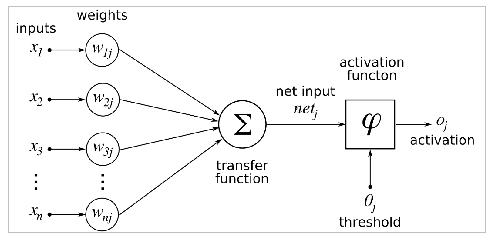
\includegraphics[width=6in]{fig/NN}}
  \caption{ANN Model}
  \label{fig:NN}
\end{figure}

ANN is considered one of the most effective methods in predicting the stock market. Even within ANN, the Multi-Layer Perceptron (MLP) model is widely accepted for effective pattern recognition. \cite{mp} An MLP model is a class of feed-forward Artificial Neural Network that consists of at least three layers of nodes namely: Input layer, Hidden layer(s) and Output layer. MLP utilizes supervised learning technique and Backpropagation algorithm for training.

The artificial neurons shown in figure \ref{fig:NN} have n number of inputs: $x_1, x_2,...,x_n$ each of which is associated with a weight onto the connection line, denoted as $w_1_j, w_2_j,...,w_n_j$ respectively. The weights can be referred as synaptic weights as in a biological neural network. '$\theta$'  represents the threshold and '$\alpha$' represents the activation function given by:

$\alpha$ = $\sum_{k = 1}^{n}  w_k_j * x_k$ + $\theta$

The output of the neuron, Oj, is a function of its activation given by:

O_j = f($\alpha$)

Several types of activation functions can be used, which are summarized in Figure \ref{fig:NNtable}:
\begin{figure}[h!]\centering
	\fbox{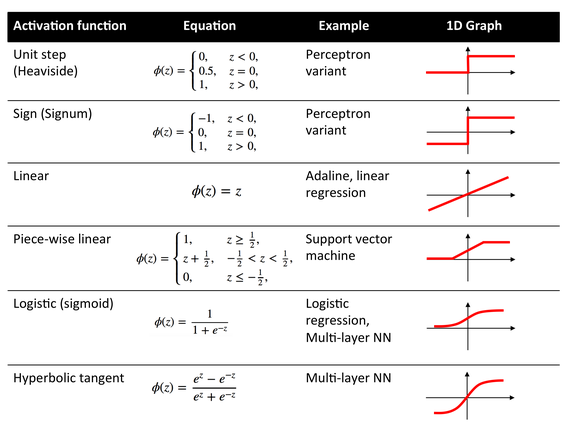
\includegraphics[width=6in]{fig/NNtable}}
	\caption{Table showing activation function}
	\label{fig:NNtable}
\end{figure}

The factors taken as input for the neural network are: 
\begin{itemize}
	\item Opening Price: the price of a company stock at the beginning of the trading day
	\item Closing Price: the price of a company stock at the end of the trading day 
	\item High Price: the maximum price reached by a company stock in the entire trading day
	\item Low Price: the minimum price reached by a company stock in the entire trading day
	\item Number of transactions: the total number of a company stock transactions within a trading day
	\item Traded Volume: the total volume of stocks traded within the entire trading day
\end{itemize}
Among the activation functions shown in figure \ref{fig:NNtable}, the Logistic (sigmoid) function is taken which best represents the non-linear feature of the dataset.

\chapter{\textbf{2. Backpropagation Algorithm }}\\
The chief objective of the Backpropagation Algorithm is to reduce the error function. \cite{ann} This algorithm falls into the general category of gradient descent algorithms, which intend to find the minima/maxima of a function by iteratively moving in the direction of the negative of the slope of the function to be minimized/maximized. This algorithm proceeds across the network, providing activation to each node until the output node is reached. Then, the weights are updated backwards, from the output layer towards the input layer until one epoch has been completed. The weights are updated according to the respective errors computed for each layer. 

\begin{figure}[h!]\centering
	\fbox{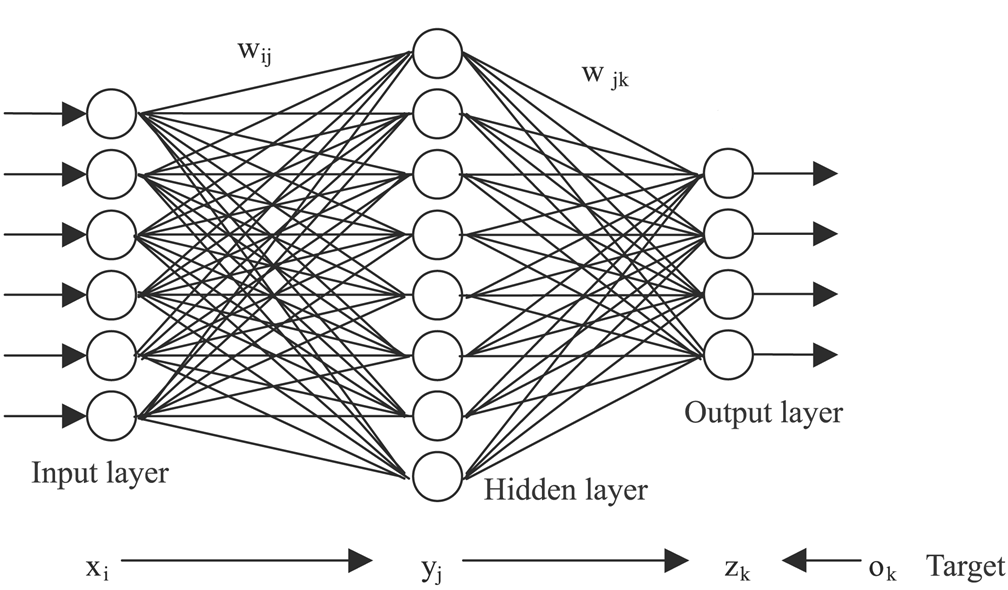
\includegraphics[width=6in]{fig/back}}
	\caption{Backpropagation Algorithm}
	\label{fig:back}
\end{figure}

Given the figure \ref{fig:back}, for k output units, if $t_{k}$ signifies the target value, $o_{k}$ signifies the actual output, $\alpha$ signifies the learning rate and $z_{ink}$ signifies the activation function for the $k^{th}$ output node, error ($\delta$) is given by:

$\delta_k$ = (t_k - o_k) * f'(z_{ink}) 

Now, the weight correction for each output unit is given by:
${\Delta}$ w_{jk} = $\alpha$ * $\delta_{k}$ * z_{j} \]

Similarly, by propagating the delta term further back in the network, the input error in the hidden network is calculated.

	$\delta_{inj}$ = $\sum_{k =1}^{m}$  $\delta_k * w_{jk}$
Where, m = number of neurons in the hidden layer

Now, error in the jth hidden unit is calculated by:
	$\delta_j$ = $\delta_{inj}$ * $f\'(x_{inj})$
Where $x_{inj}$ signifies the activation function for the $j^{th}$ hidden layer node.

Now, the weight correction is given by:

${\Delta}$ w_{ij} = $\alpha$ * $\delta_j$ * $X_i$	, for hidden layer nodes

${\Delta}$ w_{jk} = $\alpha$ * $\delta_k$ * $Y_j$	, for output layer nodes

Then, the weights for each neuron is updated with the new ones. Once an epoch has been completed, the average error for each training data is calculated. Usually the RMS error between the target value and actual outputs is computed for convergence. If the RMS error falls within the acceptable range, the training is completed, else, the whole process is repeated.

During backpropagation training, before entering the input factors in the neural network model, they are subjected to various data cleaning and pre-processing functions. The missing data are filled using interpolation techniques. The huge set of dynamic and heavily fluctuating dataset is made smooth for better calculation by taking exponential moving average (EMA) of a fixed set of data. The EMA is calculated using the formula:

EMA1 = (P* ( 2/(1+N) + [ EMA0 * ( 1-( 2/(1+N)) ])

Where, P represents price and EMA0 represents the EMA of previous calculation

Hence, the above algorithm can be used to train an Artificial Neural Network. The network, in general, can have an arbitrary number of hidden layers and an arbitrary number of hidden neurons in each layer. For practical reasons, ANNs implementing the backpropagation algorithm do not have too many layers, since the time for training the networks grows exponentially. The number of input layer neurons is decided by the number of input features in each pattern, and the number of output layer neurons is decided by the number of output features in the target values.  

There are a few disadvantages associated with backpropagation learning as well: 
\begin{itemize}
 	\item The convergence obtained from backpropagation learning is slow and not guaranteed. 
	\item The result may generally converge to any local minimum on the error surface, since stochastic gradient descent exists on a surface which is not flat. 
	\item Backpropagation learning requires input scaling or normalization. 
	\item Backpropagation requires the activation function used by the neurons to be differentiable.
\end{itemize}

\chapter{\textbf{3. K- nearest neighbor}}\\
The k-nearest neighbors algorithm is a non-parametric method used for classification and regression. \cite{Knn} It was used for classification of stock trends of individual companies in our project. The input consists of the k closest training examples in the feature space. The output in k-NN classification is a class membership. An object is classified by a majority vote of its neighbors, with the object being assigned to the class most common among its k nearest neighbors. The K-Nearest Neighbor  is a simple lazy learner algorithm that stores all available data points  and classifies new instances based on a similarity measure. It is defined by a set of objects known as examples for which the outcomes are known.

During the training phase the algorithm simply stores the data points including their class labels and all computation is deferred until the classification process. It is based on a principle that instances that are in close proximity to another have similar properties. Thus, to classify new unclassified instances, one simply has to look at their k-nearest neighbors, to figure out  the classification label. The class membership can be defined by a majority vote of the k closest neighbors or the neighbors can be ranked and weighted according to their distance to the new instance. When new case of dependent values are given k-NN finds the outcomes by finding K examples that are closest in distance to the query point.

The choice of K is very important in building the model. \cite{cho} The k is an important factor that can influence the quality of predictions. For any problem, a small value of k will lead to large variance in predictions. On the other hand setting k to a large value may lead to large model bias. Thus, k should be set to a value large enough to minimize the probability of misclassification and small enough so that the nearest points are close enough to the query point.

The KNN model is displayed in the Figure \ref{fig:KNN}.
\begin{figure}[h!]\centering
	\fbox{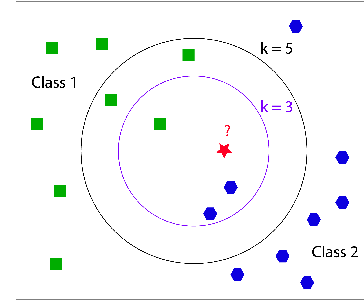
\includegraphics[width=4in]{fig/KNN}}
  	\caption{KNN model}
  	\label{fig:KNN}
\end{figure}

The neighbors are taken from a set of objects for which the class is known. This can be thought of as the training set for the algorithm, though no explicit training step is required. For this project the training set was created by making a table of six columns where the first five columns would list the difference in the closing price of that day to the previous day. The last column would however list either 1 or 0 based on whether the difference in closing price of that day to the previous day increased or decreased. Hundreds of these data would now create hundreds of classes for the test data to find a nearest neighbor from.

\subsubsection{Prediction using News Sentiment Analysis}
This system intends to predict the stock market based on the analysis of the past news
headlines. Various natural language processing and machine learning techniques are combined in order to generate the classification model. Natural language toolkit (NLTK) was used for tokenizing and pre-processing the news headlines. The processed news were then trained with the classifier and a testing model was prepared. Naive bayes classifier was used for training and testing the data.

The training set of the data was prepared in two phases. In the first phase, the news headlines relating in any way to stock market from news websites \textit{sharesansar.com} were taken for training set. The news headlines from May 2016 to June 2017 were taken for training set. The headlines were classified at first, on the basis of the next day's nepse index value. If the value of nepse index increased, then all the news from previous day were considered as positive news and vice versa.  But the classification was not enough to generate good prediction hence further refinement was necessary. In second phase of classification, these classified news headlines were classified manually. Manual classification involved reading each news headlines and assigning it a sentiment tag: positive, negative or neutral. The second phase of the classification needed much research on the minute details. 

Now a refined dataset was prepared for training the classifier. News headlines from past two days are collected as an unknown test dataset. The classifier predict the increment/decrement of NEPSE index by calculating the total number of positive, negative and neutral news headlines.

\chapter{\textbf{1. Text preprocessing}} \\
News headlines are unstructured data and these data needs preprocessing to input into classifier. For text preprocessing, sentence tokenizer and word tokenizer from NLTK modules were used. \textbf{Tokenizer} is used to divide strings into lists of substrings.\textbf{Sentence tokenizer} is used to find the list of sentences and \textbf{word tokenizer} is used to find the list of words in strings. After tokenizing, stop words were removed from the words. \textbf{Stop words} are the words that are to be filtered out before training the classifier. These are usually high frequency words that aren't giving any additional information to our labelling. In fact, they actually confuse the classifier. Example: is, the, at, etc.

\chapter{\textbf{2. Sentiment Detection}}  \\
\cite{na} For the sentiment detection of news articles, dictionary based approach is being followed which uses Bag of Word techniques for text mining. This method is based on the research of \cite{jb} J. Bean in his implementation of Twitter sentiment analysis for airline companies. From Bag of Word model, the features from news headlines are extracted and the features from model and the sentiment for each news headlines are inputed into naive bayes classifier for training the classifier. Then a test dataset is inputed to the classifier to predict the sentiments from the news headlines.

\chapter{\textbf{i. Bag of Words}} \\
The Bag of Words model is a simplifying representation used in natural language processing and information retrieval. In this model , a text is represented as the bag of its words, disregarding grammar and even word order but keeping multiplicity. The Bag of Words model learns a vocabulary from all of the documents, then models each document by counting the number of times each word appears. 

For example, consider the following two sentences:

Sentence 1: "The cat sat on the hat"

Sentence 2: "The dog ate the cat and the hat"

From these two sentences, our vocabulary is as follows:
{ the, cat, sat, on, hat, dog, ate, and }

To get the bags of words, the number of times each word occurs in each sentence is counted. In Sentence 1, "the" appears twice, and "cat", "sat", "on", and "hat" each appear once, so the feature vector for Sentence 1 is: 

{ the, cat, sat, on, hat, dog, ate, and }

Sentence 1: { 2, 1, 1, 1, 1, 0, 0, 0 }

Similarly, the features for Sentence 2 are: { 3, 1, 0, 0, 1, 1, 1, 1}

The feature extraction module from scikit-learn is used to create bag-of-words features.

\chapter{\textbf{ii. Naive Bayes Classifier}}\\
\cite{nbb} Naive Bayes is a classification technique based on Bayes Theorem with an assumption of independence among predictors. In simple terms, a Naive Bayes classifier assumes that the presence of a particular feature in a class is unrelated to the presence of any other feature. For example, a fruit may be considered to be an apple if it is red, round, and about 3 inches in diameter. Even if these features depend on each other or upon the existence of the other features, all of these properties independently contribute to the probability that this fruit is an apple and that is why it is known as 'Naive'.
Naive Bayes model is easy to build and particularly useful for very large data sets. Along with simplicity, Naive Bayes is known to outperform even highly sophisticated classification methods.
Bayes theorem provides a way of calculating posterior probability P(c|x) from P(c), P(x) and P(x|c).

Look at the equation \ref{fig:naive},

\begin{figure}[h!]\centering
	\fbox{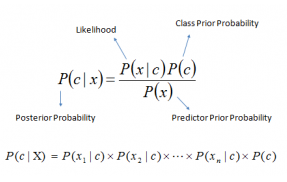
\includegraphics[width=3in]{fig/naive}}
	\caption{Equation of Bayes theorem}
	\label{fig:naive}
\end{figure}

Where,
	P(c|x) is the posterior probability of class(c,target) give predictor(x, attributes).

	P(c) is the prior probability of class.

	P(x|c) is the likelihood which is the probability of predictor given class.
	
	P(x) is the prior probability of predictor.

\chapter{\textbf{Pros and Cons of Naive Bayes Classifier :}}\\
\chapter{\textbf{Pros:}}
\begin{itemize}
	\item It is easy and fast to predict class of test data set. It also perform well in multi-class prediction
	\item When assumption of  independence holds, a Naive Bayes classifier performs better compared to other models like logistic regression and you need less training data.
	\item It perform well in case of categorical input variables compared to numerical variable(s). For numerical variable, normal distribution is assumed (bell curve, which is a strong assumption).
\end{itemize}

\chapter{\textbf{Cons}}
\begin{itemize}
	\item If categorical variable has a category (in test data set), which was not observed in training data set, then model will assign a 0 (zero) probability and will be unable to make a prediction. This is often known as "Zero Frequency". To solve this, the smoothing technique can be used. One of the simplest smoothing techniques is called Laplace estimation.
	\item Another limitation of Naive Bayes is the assumption of independent predictors. In real life, it is almost impossible to get a set of predictors which are completely independent.
\end{itemize}

Scikit learn (python library) also help to build a Naive Bayes model in Python. There are three types of Naive Bayes model under scikit learn library:
\begin{itemize}
	\item \textbf{Gaussian :} It is used in classification and it assumes that features follow a normal distribution.
	\item \textbf{Multinomial :} It implements the naive Bayes algorithm for multinomially distributed data, and is one of the two classic naive Bayes variants used in text classification (where the data are typically represented as word vector counts, although tf-idf vectors are also known to work well in practice). 
	\item \textbf{Bernoulli :} The binomial model is useful if your feature vectors are binary (i.e. zeros and ones). One application would be text classification with 'bag of words' model where the 1s \& 0s are "word occurs in the document" and "word does not occur in the document" respectively.
\end{itemize}
